\begin{figure}
  \centering
  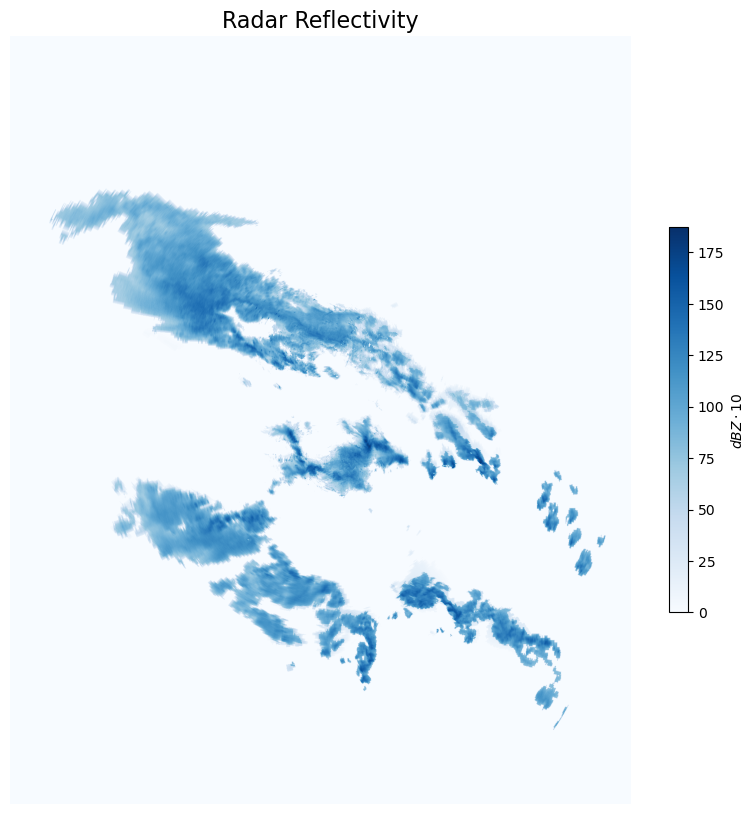
\includegraphics[width=225pt]{./images/radar_reflectivity.png}
  \caption{Radar Reflectivity}
  \Description{}
  \label{fig:reflect}
\end{figure}

\begin{figure}
  \centering
  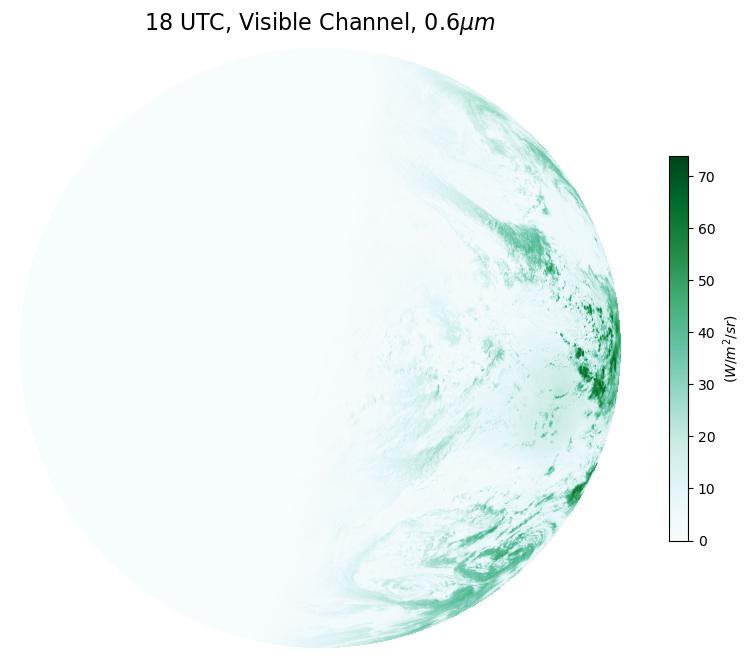
\includegraphics[width=225pt]{./images/vis_006.png}
  \caption{Satellite Image: Visible Channel 18UTC $0.6\mu m$}
  \Description{}
  \label{fig:vis}
\end{figure}

\begin{figure}
  \centering
  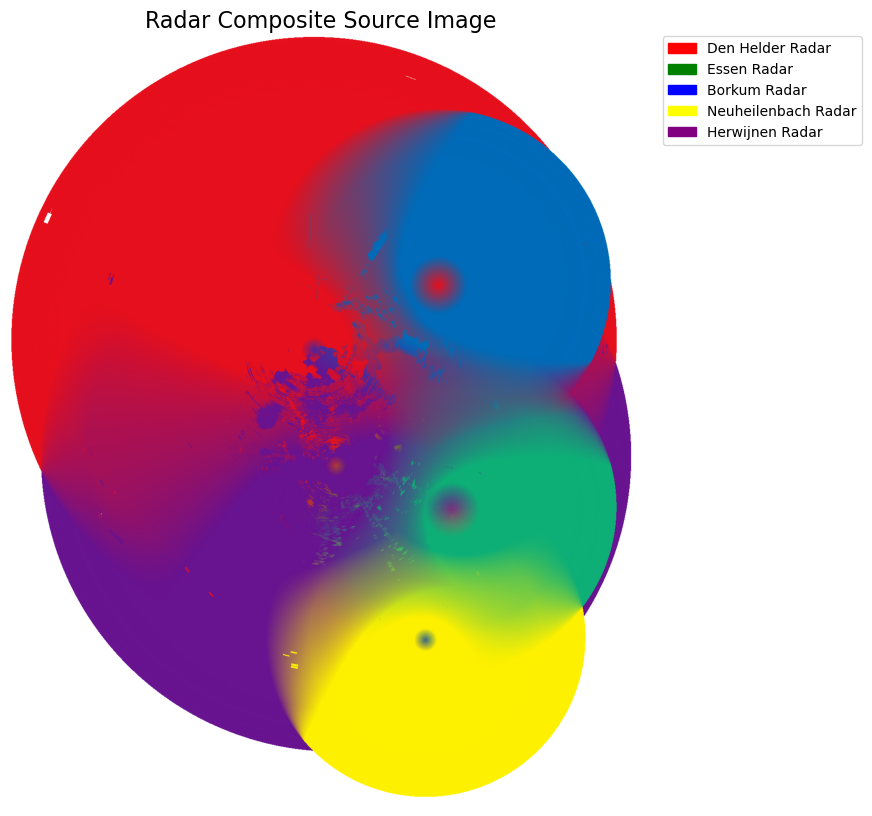
\includegraphics[width=225pt]{./images/radar_source.png}
  \caption{Satellite Image: Infrared Channel 18UTC $12.0\mu m$}
  \Description{}
  \label{fig:source}
\end{figure}

\begin{table}[]
  \caption{Available Satellite Channels.}
  \begin{tabular}{@{}lll@{}}
  \toprule
  Channel & Type        & $\lambda$ \\ \midrule
  VIS006  & Visual      & 0.6 mm      \\
  VIS008  & Visual      & 0.8 mm      \\
  IR\_016 & Infrared    & 1.6 mm      \\
  IR\_039 & Infrared    & 3.9 mm      \\
  IR\_087 & Infrared    & 8.7 mm      \\
  IR\_097 & Infrared    & 9.7 mm      \\
  IR\_108 & Infrared    & 10.8 mm     \\
  IR\_120 & Infrared    & 12.0 mm     \\
  IR\_134 & Infrared    & 13.4 mm     \\
  WV\_062 & Water Vapor & 6.2 mm      \\
  WV\_073 & Water Vapor & 7.3 mm      \\ \bottomrule
  \end{tabular}
  \label{tab:channels}
\end{table}

\begin{table}[h]
\caption{Reflectivity in dBZ versus Rainrate}
\begin{tabular}{@{}llll@{}}
\toprule
LZ(dBZ) & R(mm/h) & R(in/h)        & Intensity             \\ \midrule
5       & (mm/h)  & \textless 0.01 & Hardly noticeable     \\
10      & 0.15    & \textless 0.01 & Light mist            \\
15      & 0.3     & 0.01           & Mist                  \\
20      & 0.6     & 0.02           & Very light            \\
25      & 1.3     & 0.05           & Light                 \\
30      & 2.7     & 0.10           & Light to moderate     \\
35      & 5.6     & 0.22           & Moderate rain         \\
40      & 11.53   & 0.45           & Moderate rain         \\
45      & 23.7    & 0.92           & Moderate to heavy     \\
50      & 48.6    & 1.90           & Heavy                 \\
55      & 100     & 4              & Very heavy/small hail \\
60      & 205     & 8              & Extreme/moderate hail \\
65      & 421     & 16.6           & Extreme/large hail    \\ \bottomrule
\end{tabular}
\end{table}

\begin{listing}
  \begin{minted}{toml}
    [model]
    name = "SAT2RAD_UNET"
    classes=8
    
    [model.input_size]
    height = 256
    width = 256
    channels = 12
    sequence_length = 8
    
    [model.output_size]
    height = 256
    width = 256
    channels = 1
    sequence_length = 1
    
    [model.unet]
    kernel_size = [3, 3]
    layers = 3
    filters = 64
    
    [model.training]
    max_epochs = 100
    class_weights = [
                0.01081153,
                0.13732371,
                0.13895907,
                0.1416087,
                0.14272867,
                0.14285409,
                0.14285709,
                0.14285714,
            ]
    metrics = [
        'acc',
        'precision',
        'recall',
        'exact',
        'f1', 
        'jaccard'
    ]
    
    [mlflow]
    experiment_name = "sat2rad_unet"
    experiment_tracker = "Infoplaza MLFlow"
    
    
    [visualize]
    output_dir = '../../../../../logs/'
  \end{minted}
  \caption{toml configuration file for U-Net Model.}
  \label{lst:hello}
\end{listing}